\documentclass[main]{subfiles}


\begin{document}
\newpage
\section{Deep Learning With Spikes}


\subsection{Motivation}
Neurobiology mostly uses spiking neural networks. Neurons output spikes, which are binary events and localized in time. 

So how do hidden units learn?
\paragraph{Bottom-up approach:}
\begin{itemize}
    \item Start with a random network model
    \item Include data driven plasticity model
    \item Observe function $\rightarrow$ Limited success in learning useful hidden layer representations
\end{itemize}
One outcome would be Spike-time dependent plasticity (STDP), which is a way the weights can be adjusted. So far not very useful in building networks; the weights tend to blow up. Over the years, people went over this concept and tried to improve. 

\paragraph{Top-down approach:}
\begin{itemize}
    \item Start with function in mind
    \item Derive suitable plasticity rules
    \item Build functional network models
\end{itemize}
Deep learning is an example of a top-down framework. Two questions remain: 

\textbf{The algorithmic question:} How to compute the gradient?

\textbf{The conceptual question:} Which functions are learned?

\begin{figure}[H]
    \centering
    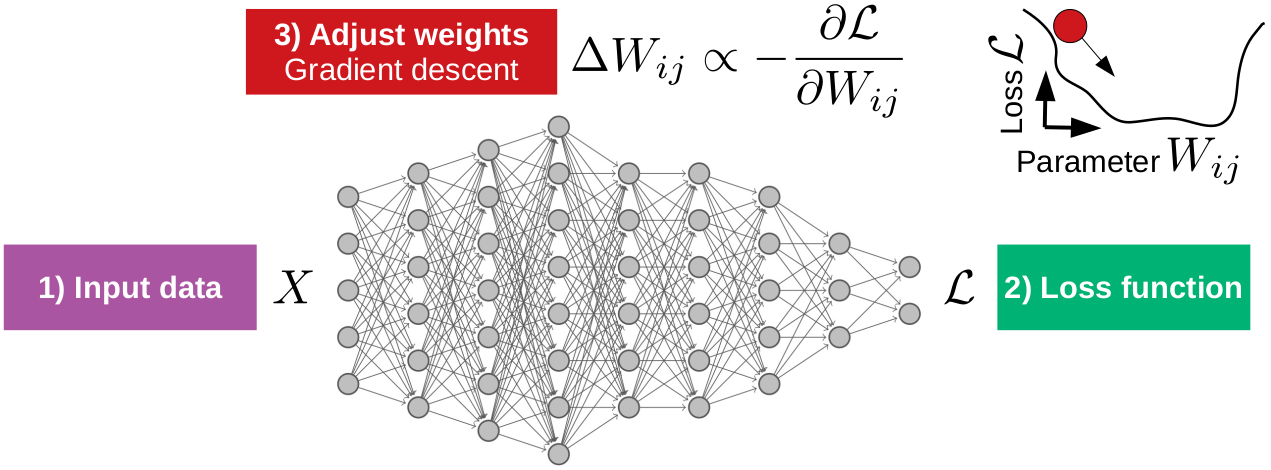
\includegraphics[width=0.95\linewidth]{10_DeepLearningWithSpikes/figures/deeplearning.png}
    \caption{Deep learning as a top-down framework}
    \label{fig:my_label}
\end{figure}

\subsection{Recap: Spiking Neuron Models}
\begin{figure}[H]
    \centering
    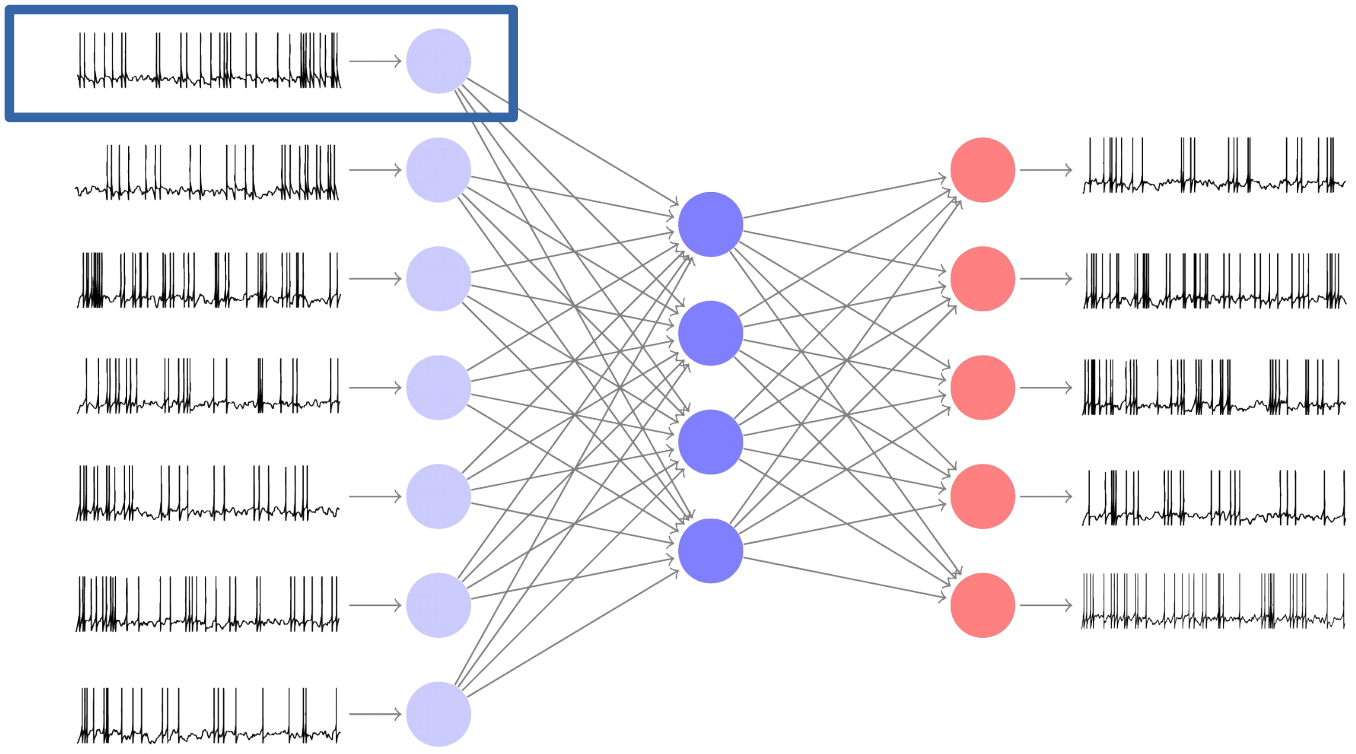
\includegraphics[width=0.8\linewidth]{10_DeepLearningWithSpikes/figures/snn.png}
    \caption{Illustration of a Spiking Neural Network}
    \label{fig:my_label}
\end{figure}

\begin{itemize}
    \item Spiking networks consist of spiking neurons
    \item Network modeling largely relies on simplified neuron models
\end{itemize}

\subsubsection{Biophysics of neuronal signal transmission}
\begin{figure}[H]
    \centering
    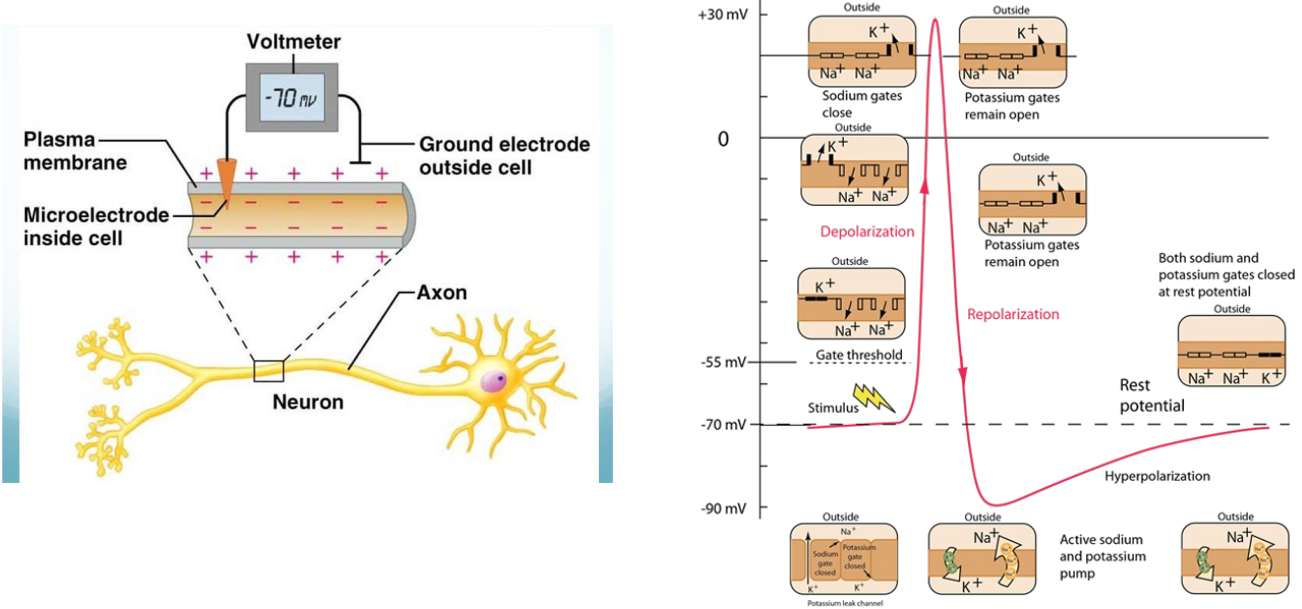
\includegraphics[width=0.99\linewidth]{10_DeepLearningWithSpikes/figures/biophysics.png}
    \caption{}
    \label{fig:my_label}
\end{figure}

\subsubsection{From biophysical to reduced neuron models}
In order to build a phenomenological model of neuronal dynamics\footnote{Incredibly useful and free book by Wulfram Gernster et. al, where most of the content of this section is copy-pasted from: \url{https://neuronaldynamics.epfl.ch/online/index.html}}, we describe the critical voltage for spike initiation by a formal threshold $\theta$. If the voltage $U_i(t)$ (that contains the summed effect of all inputs) reaches $\theta$ from below, we say that neuron $i$ fires a \textbf{spike}. The moment of threshold crossing defines the firing time $t^{(f)}_i$. 
The model makes use of the fact that neuronal action potentials of a given neuron always have roughly the same form. If the shape of an action potential is always the same, then the shape cannot be used to transmit information: rather information is contained in the presence or absence of a spike. Therefore action potentials are reduced to ‘events’ that happen at a precise moment in time.



\paragraph{Leaky integrate-and-fire neuron: }
Neuron models where action potentials are described as events are called 'Integrate-and-Fire' models. No attempt is made to describe the shape of an action potential. Integrate-and-fire models have two separate components that are both necessary to define their dynamics:
\begin{enumerate}
    \item An equation that describes the evolution of the membrane potential $U_i(t)$
    \item A mechanism to generate spikes.
\end{enumerate}
The variable $U_i$ describes the momentary value of the membrane potential of neuron $i$. In the absence of any input, the potential is at its resting value $U_{rest}$. If an experimentalist injects a current $I(t)$ into the neuron, or if the neuron receives synaptic input from other neurons, the potential $U_i(t)$ will be deflected from its resting value. The basic electrical circuit representing a leaky integrate-and-fire model consists of a capacitor $C$ in parallel with a resistor $R$ driven by a current $I(t)$, as shown in the figure below. The differential equation for describing the leaky-integration of the voltage is given by
%
\begin{equation}
\tau \frac{\mathrm{d}}{\mathrm{d} t} U(t)=-\left(U(t)-U_{\mathrm{rest}}\right)+R_{\mathrm{in}} I(t),
\end{equation}
where $\tau = RC$ is the time constant of the circuit. 
%
\begin{figure}[H]
    \centering
    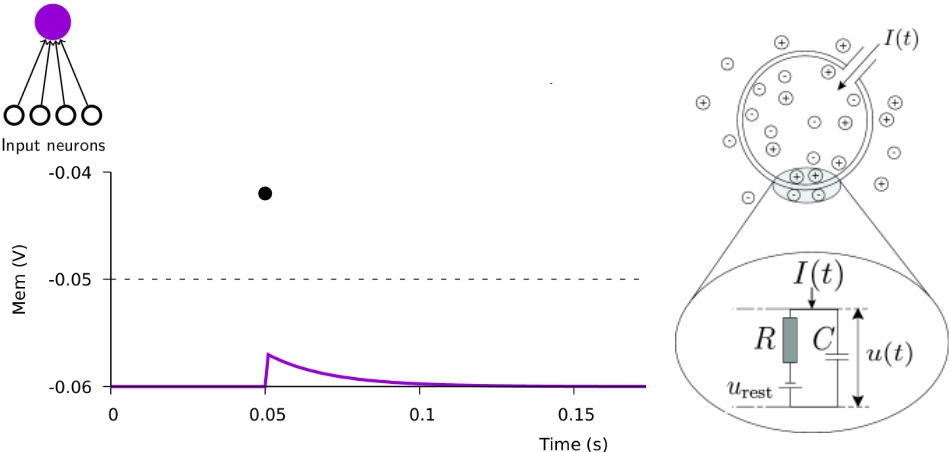
\includegraphics[width=0.8\linewidth]{10_DeepLearningWithSpikes/figures/passive_membrane.png}
    \caption{Passive Membrane}
    \label{fig:my_label}
\end{figure}
%
Now the second part of the leaky integrate-and-fire neuron is the firing and re-setting of the voltage after the neuron-specific threshold has been reached. At the firing time $t^{f}: U(t^{f}) = \theta$, the neuron fires (with a not-here-to-be-defined spike-form), the firing time is noted and immediately after the voltage reset to a new value $U_rest < \theta$:
\begin{equation}
    \lim_{\delta \to 0; \delta > 0} U(t^{(f)} + \delta) = U_{rest}
\end{equation}
%
\paragraph{}
\begin{figure}[H]
    \centering
    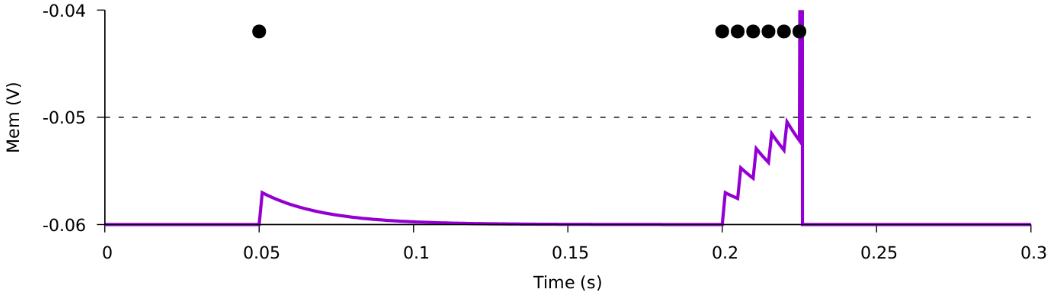
\includegraphics[width=0.6\linewidth]{10_DeepLearningWithSpikes/figures/leaky_ifn.png}
    \caption{}
    \label{fig:my_label}
\end{figure}
%
\paragraph{Exponential postsynaptic currents: }
\hl{?? Please help, I don't really get it}
We also want to model the synapse. The following differential equation describes the evolution of the postsynaptic current $I(t)$:
%
\begin{equation}
\frac{\mathrm{d}}{\mathrm{d} t} I(t)=-\frac{I(t)}{\tau_{\mathrm{syn}}}+S(t)
\end{equation}
%
\begin{figure}[H]
    \centering
    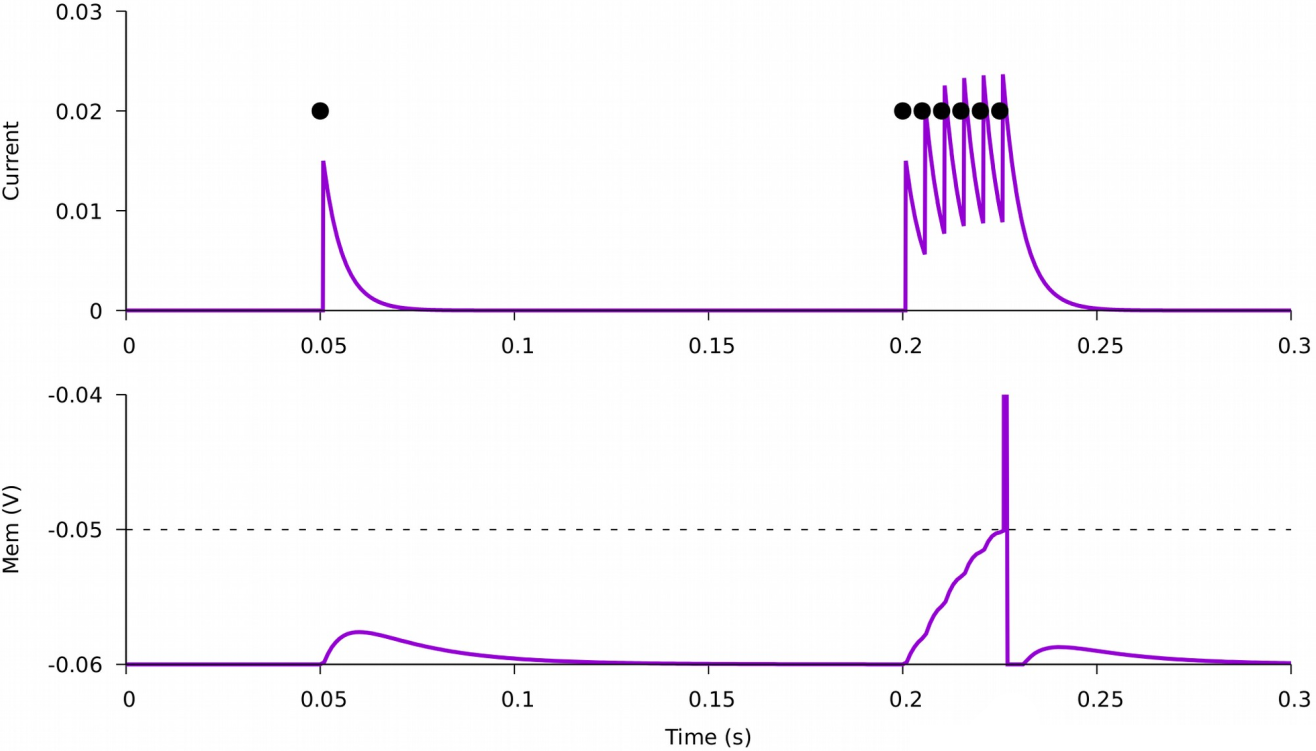
\includegraphics[width=0.55\linewidth]{10_DeepLearningWithSpikes/figures/exp_ps_current.png}
    \caption{}
    \label{fig:my_label}
\end{figure}
%
\paragraph{The spike response model (SRM):}
\hl{?? Also here}
So far, we have described neuronal dynamics in terms of systems of differential equations. There is another approach called the ‘filter picture’. In this picture, the parameters of the model are replaced by (parametric) functions of time, generically called ‘filters’. The neuron model is therefore interpreted in terms of a membrane filter as well as a function describing the shape of the spike and, potentially, also a function for the time course of the threshold. Together, these three functions establish the Spike Response Model (SRM).
Mathematically speaking, we integrate over the differential equation, then replace the integration times multiplications with convolutions of filter kernels over the spikes:
%
\begin{equation}
\mathrm{U}_{i}(t)=\sum_{j} w_{i j}\left(\epsilon * S_{j}\right)(t)+\left(\eta * S_{i}\right)(t)+U_{\mathrm{rest}}
\end{equation}
%
\begin{figure}[H]
    \centering
    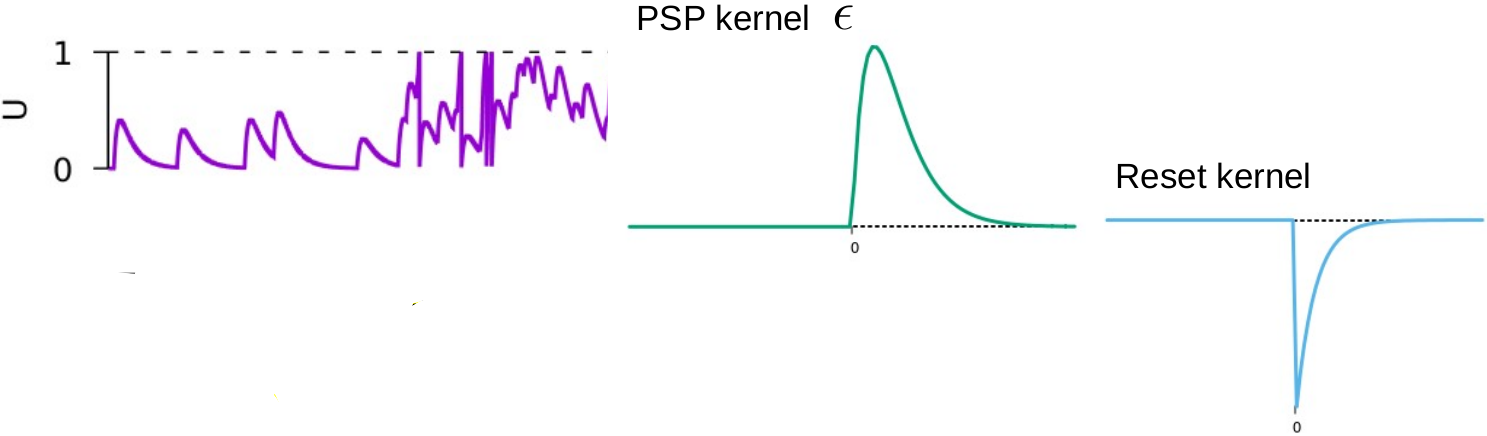
\includegraphics[width=0.7\linewidth]{10_DeepLearningWithSpikes/figures/spike_response_model.png}
    \caption{}
    \label{fig:my_label}
\end{figure}
%
\paragraph{Towards functional neural network models: }
We want this
\begin{figure}[H]
    \centering
    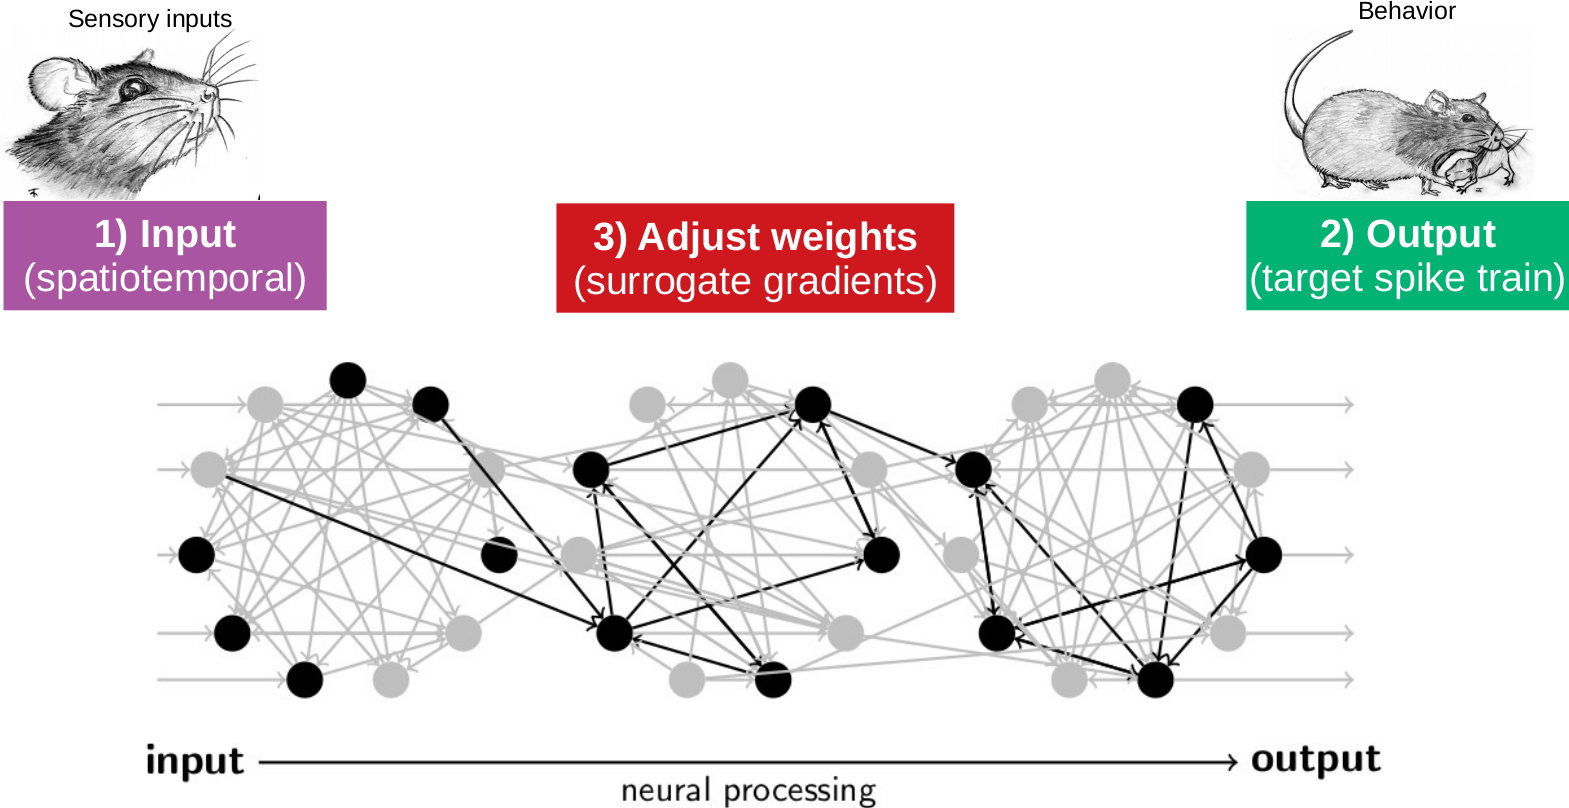
\includegraphics[width=0.8\linewidth]{10_DeepLearningWithSpikes/figures/towards_functional_nn.png}
    \caption{}
    \label{fig:my_label}
\end{figure}

\subsection{Dealing with the Vanishing Gradient Problem}

\subsubsection{Defining the problem}
Can we do supervised learning in spiking multi-layer networks with a local online learning rule? We want to compare output spikes with target spikes. Let's try:
\paragraph{Van Rossum distance between output and target spike trains:}
There is different ways of representing a spike train. If the spikes are seen to be discrete units, the spike train $S(t)$ is given simply by
%
\begin{equation}
    S_{\delta}(t) = \sum_i^M \delta_{VR}(t-t_i)
\end{equation}
%
Replacing the delta function associated with each spike with an exponential function, that is, add an exponential tail to all spikes, leads to
%
\begin{equation}
    S(t) = \sum_i^M H(t-t_i)\exp{-(t-t_i)/t_c},
\end{equation}
%
where $H(t)$ is the heavyside function. Then, the loss between the target spikes distance $\hat{S}$ and the output spikes distance $S$ can be defined as the Van Rossum distance:
%
\begin{equation}
\mathcal{L}=\frac{1}{2} \int_{-\infty}^{t}[\lambda *(\hat{S}(s)-S(s))]^{2} ds
\end{equation}
%
The problem with our spike model and such a loss becomes evident when we try to differentiate the loss with respect to the single weights:
%
\begin{equation}
-\frac{\partial \mathcal{L}}{\partial w_{k}}=\int_{-\infty}^{t} \lambda *(\hat{S}(s)-S(s)) \lambda * \frac{\partial S(t)}{\partial w_{k}} d s
\end{equation}
%
The partial derivation $\frac{\partial S(t)}{\partial w_{k}}$ This derivative is problematic because for most neuron models, it is zero except at spike times at which it is not defined. Thus it forces the gradient to vanish. 
%
\begin{figure}[H]
    \centering
    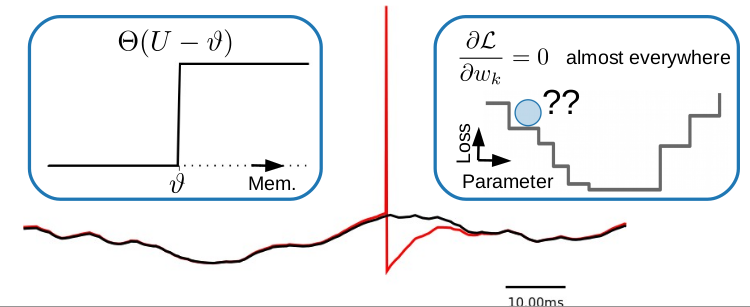
\includegraphics[width=0.8\linewidth]{10_DeepLearningWithSpikes/figures/vanishing.png}
    \caption{}
    \label{fig:my_label}
\end{figure}
%

\subsubsection{A history of struggle}

\paragraph{Noise injection :}\footnote{Pfister, Toyoizumi, Barber \& Gerstner (2006), Gardner, Sporea & Grüning (2015)} \hl{Write smth here.}

\paragraph{Differentiate firing times :}\footnote{Bohte, Kok, & Poutre (2002), Gütig \& Sompolinski (2006), Gütig (2016), Mostafa (2018)} (skipped in lecture)

\paragraph{Make spikes differentiable :}\footnote{Huh \& Sejnowski (2018)}

\paragraph{Force hidden units "on target" :}\footnote{Gilra \& Gerstner (2017), Nicola & Clopath (2017)}

\paragraph{e.g. firing-rate approaches :}\footnote{Hunsberger \& Eliasmith (2015), Lee et al. (2016), ...}

\newpage
\subsubsection{Surrogate gradients \& SuperSpike}
Idea\footnote{Zenke \& Ganguli, "SuperSpike: Supervised Learning in Multilayer Spiking Neural Networks", 2018}: Replace the non-differentiable heaviside function with the differentiable sigmoid function $\sigma$, but only in the backward-pass. In the forward pass, leave it as a heaviside function. The equivalent in machine learning would be "Straight-through estimators"\footnote{Begio et al., "Estimating or Propagating Gradients Through Stochastic Neurons for Conditional Computation", 2013}. This procedure leads to the replacements:
%
\begin{equation}
\frac{\partial S_{i}}{\partial w_{i j}} \quad \rightarrow \quad \sigma^{\prime}\left(U_{i}\right) \frac{\partial U_{i}}{\partial w_{i j}}
\end{equation}
%
\begin{figure}[H]
    \centering
    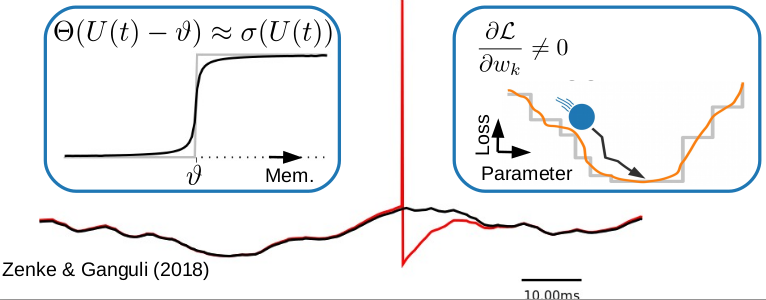
\includegraphics[width=0.8\linewidth]{10_DeepLearningWithSpikes/figures/surrogate_gradient.png}
    \caption{}
    \label{fig:my_label}
\end{figure}
%
If now the membrane potential $U_i(t)$ is written in the integral form as a spike response model ($SRM_0$)
%
\begin{equation}
\mathrm{U}_{i}(t)=\sum_{j} w_{i j}\left(\epsilon * S_{j}\right)(t)+\left(\eta * S_{i}\right)(t)+U_{\mathrm{rest}}, 
\end{equation}
%
where $\epsilon$ is the causal membrane kernel (corresponding to the postsynaptic potential) and $\eta$ captures spike dynamics and reset. With some steps that are briefly explained in the paper, one gets for the gradient descent learning rule for a single neuron the following expression:
%
\begin{equation}
\frac{\partial w_{i j}}{\partial t}=r \int_{-\infty}^{t}  \lambda *( \underbrace{\left(\epsilon * S_{j}\right)(s)}_{\text {Pre }} \underbrace{\sigma^{\prime}\left(U_{i}(s)\right)}_{\text {Post }}) \underbrace{e_{i}(s)}_{\text {Error signal }} ds
\end{equation}
%
Here, $r$ is the learning rate, $e_{i}(s)=\lambda*(\hat{S_i}-S_i)$ the error signal and $\lambda$ the eligibility trace ("Ca transient"). This learning rule is called \textbf{SuperSpike}. We can divide this rule into three factors:
%
\begin{itemize}
    \item[\textbf{Pre}] Presynaptic activity
    \item[\textbf{Post}] Postsynaptic activity
    \item[\textbf{Error signal}] Specific feedback
\end{itemize}
%
The pre- and postsynaptic activity are combined in a multiplicative manner, which can be seen as the Hebbian term (which is "STDP"-like). $\sigma^'$ is the voltage nonlinearity, thus the learning rule is voltage based. 

\subsubsection{Hidden layers}
What about training the hidden layers? The learning rule for hidden weights is 
%
\begin{equation}
\frac{\partial w_{i j}}{\partial t} \equiv \sum_{k} e_{k}(t) \epsilon *\left[w_{k i} \epsilon *\left(\epsilon * S_{j}(t) \sigma^{\prime}\left(U_{i}\right)\right) \sigma^{\prime}\left(U_{k}\right)\right].
\end{equation}
%
Biologically seen this is problematic, because
\begin{enumerate}
    \item It requires symmetric weights
    \item There are downstream activities
\end{enumerate}
One way to overcome those issues is by applying feedback-alignment, which is well documented in \cref{sec:training}. Note that all quantities computed online. Temporal credit assignment through dynamics at the synaptic level (eligibility trace).

\begin{figure}[H]
    \centering
    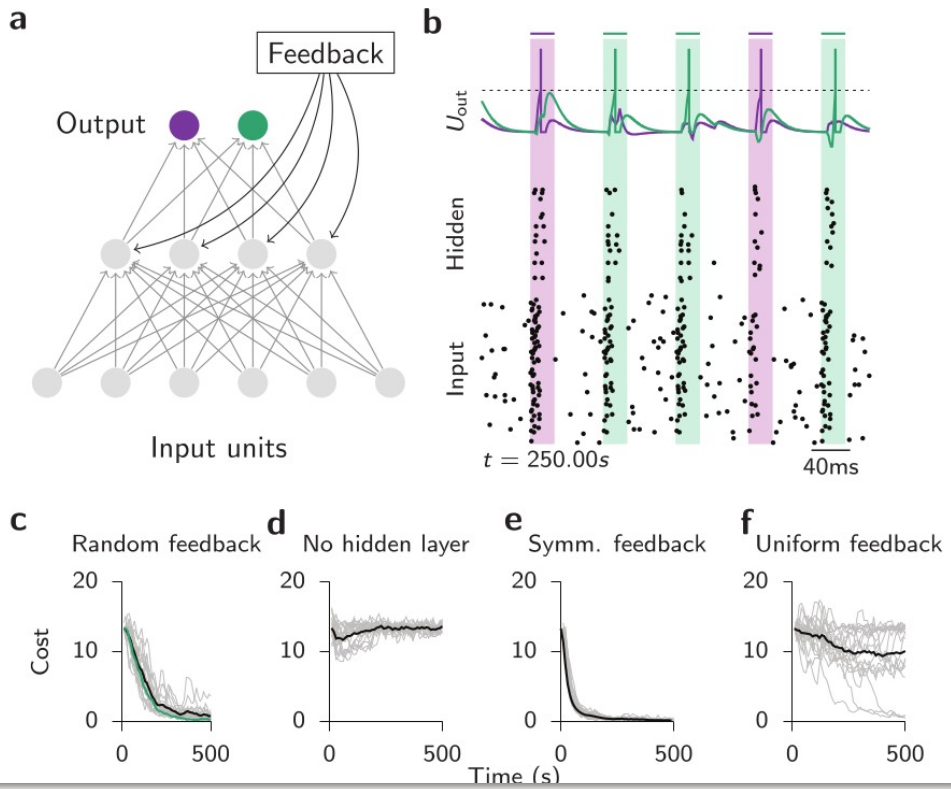
\includegraphics[width=0.8\linewidth]{10_DeepLearningWithSpikes/figures/feedbackalignment.png}
    \caption{Network trained to solve a nonlinearly separable classification problem with noisy input neurons. \textbf{(a)} Sketch of network layout with two output units and four hidden units. \textbf{(b)} Snapshot of network activity at the end of training with random feedback. Four input patterns from two nonlinearly separable classes are presented in random order (shaded areas). In between stimulus periods, input neurons spike randomly with 4 Hz background firing rate. \textbf{(c)} Learning curves of 20 trials with different random initializations (gray) for a network with random feedback connections that solves the task. The average of all trials is given by the black line. The average of 20 simulation trials with an additional regularization term (see section 3) is shown in green. \textbf{(d)} Same as panel c but for a network without hidden units that cannot solve the task. \textbf{(e)} Same as panel c but for symmetric feedback. \textbf{(f)} Same as panel c but for uniform ("all ones") feedback connections.}
    \label{fig:my_label}
\end{figure}


\subsubsection{Sequence-to-sequence learning}

\subsection{Spiking nets and temporal coding}

\end{document}